\chapter{Iterative Learning Control}
\label{chapter4}

In Chapters 2 and 3, a steering controller and trajectory planning algorithm were presented for an autonomous race car. One of the goals
from the introduction was to compare the resulting autonomous driving performance with that of a human driver. While there are
several metrics that could be used as a comparison, by far the easiest to measure and most relevant for racing is lap time. Figure
\ref{fig:expLT} shows lap times recorded on the Audi TTS, both autonomously and from two human drivers. One of the human drivers is a professional race
driver, while the other is an expert amateur driver. 

\begin{figure}[tb]
\centering
\includegraphics[width=.9\fullwidth]{expLT.png}
\caption{Experimentally recorded lap times (in seconds).}
\label{fig:expLT}
\end{figure}

While the lap times from the autonomous driver are comparable to the amateur expert, they are about a second behind on average from the professional
human driver. There are several ways to analyze why this difference arises, but a simple insight that makes the case for learning algorithms comes
from viewing the trajectory tracking performance and friction utilization of the controller, shown in Fig.~\ref{fig:expErrors}.

\begin{figure}
\centering
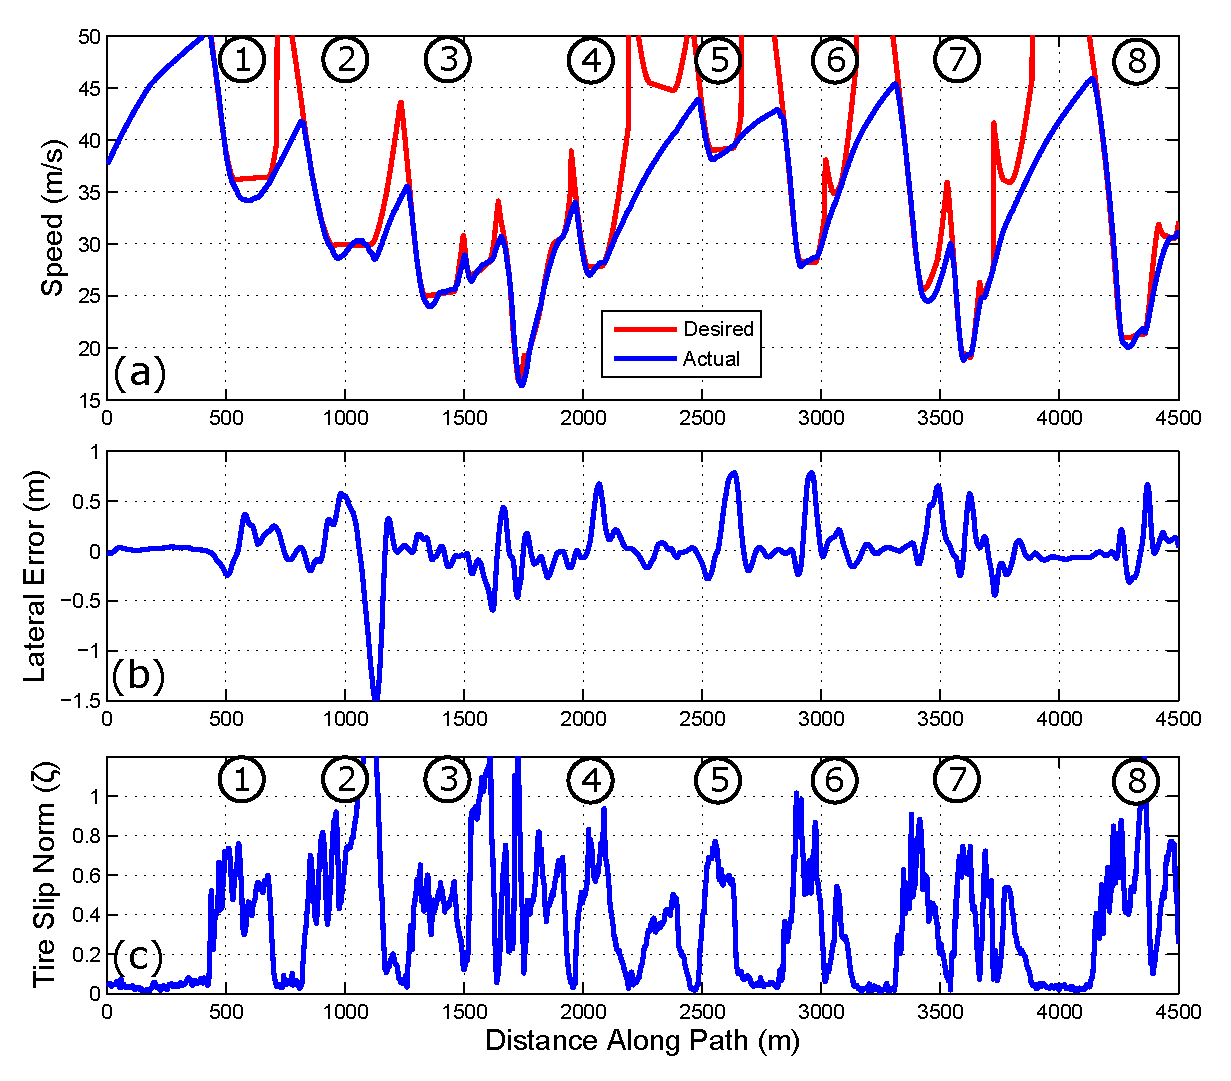
\includegraphics[width=\fullwidth]{expErrors.eps}
\caption{Controller tracking performance and tire slip norm on a test run at the limits of handling ($\mu =$ 0.95).(a) Desired
vs actual speed of the vehicle. (b) Lateral tracking error and (c) tire slip norm as a function of distance along the path.}
\label{fig:expErrors}
\end{figure}

One of the issues shown in Fig.~\ref{fig:expErrors} is the relatively poor controller tracking on a few sections of the race track. While
this is probably less significant for the lateral speed tracking (sections \circled{2}, \circled{4} - \circled{7}), failing to drive as fast as the trajectory plans (sections \circled{1}, \circled{2}, \circled{7}) results directly in a loss 
of lap time. The speed and lateral path tracking will be improved in this chapter with the addition of iterative learning control
(ILC) algorithms. 

The second issue shown in Fig.~\ref{fig:expErrors} is the inconsistent usage of the tire friction capacity, as judged by the tire slip norm metric.
The tire slip norm, formalized in \cite{mickthesis}, is given by $\zeta$:

\begin{equation}
\label{eq:zeta}
\zeta = \sqrt{\left(\dfrac{\alpha}{\alpha_{p}}\right)^2 + \left(\dfrac{\sigma}{\sigma_p}\right)^2}
\end{equation}

Where $\sigma$ and $\alpha$ are the longitudinal and lateral tire slip for a given tire, and $\sigma_p$ and $\alpha_p$ are empirically
determined \textit{peak slip} values resulting in maximum longitudinal and lateral tire force generation. As a result, $\zeta < 1 $ corresponds to the tires having
excess force generation capacity, while $\zeta > 1$ corresponds to tire saturation. There is technically a $\zeta$ value for each tire, but the maximum
$\zeta$ over all four tires is typically used for conservatism. 

Fig.~\ref{fig:expErrors} shows inconsistent usage of tire friction across many turns. On some turns (sections \circled{2} and \circled{8}), the vehicle significantly exceeds
the limits of handling, and the car's stability control systems kick in to regain control, slowing the car down in the process. On other turns (sections \circled{3}, \circled{5}, and \circled{7}),
the vehicle uses only a portion of the available tire force, indicating the vehicle can actually drive with higher acceleration on the next lap. 
Learning from prior runs to find the optimal acceleration (or $\mu$ parameter) for each part of the track will be accomplished in the next chapter via a search algorithm. 

\subsubsection{Iterative Learning Control}

Iterative learning control (ILC) is based on the notion that the performance of a system that executes the
\textit{same task} multiple times can be improved by learning from previous executions (trials, iterations, or in our case, laps of racing) \cite{bristow}.
On every iteration, a control signal is applied to a system in order to follow an ideal, unchanging ``reference trajectory". 
The tracking error for that iteration is recorded, and a learning algorithm is applied to improve the control signal and achieve
more accurate system performance on the next iteration. There are a variety of learning algorithms used, but most attempt to correct the tracking
error by using a model of the system to determine the augmentation to apply to the prior control signal. This process is repeated until the reference tracking performance becomes satisfactory.
As noted by Bristow et al., this approach is analogous to how a basketball player shooting a free throw from a fixed position can improve her ability to
score by practicing the shot repeatedly, making adjustments to her shooting motion based on observations of the ball's trajectory \cite{bristow}.

Inspired by a series of papers published in 1984 \cite{arimoto}\cite{craig}\cite{kawamura}, iterative learning control has become increasingly widespread. Because
iterative learning control works best when learning to follow the same reference trajectory under the same ambient conditions, the most common applications
of ILC are in the field of automated manufacturing. Notable examples include CNC machining \cite{kimdi}, industrial robotics \cite{freeman}\cite{hladowski}, piezolectric stage
positioning \cite{huang}, motor control \cite{mohammad}, and microdeposition \cite{hoelzle}. However, the rise of automated systems outside
factory environments has led to important applications of ILC for ground and air robotics. In 2006, Chen and Moore \cite{chen} proposed
 a simple iterative learning scheme in 2006 to improve path-following of a ground vehicle with omni-directional wheels. In 2011, Purwin and Andrea synthesized
 an iterative controller using least-squares methods to aggressively maneuver a quadrotor
 unmanned aerial vehicle (UAV) from one state to another \cite{purwin}. As a novel step, the authors then generalized the experience learned
 from the iterative learning control in order to tune the parameters of the UAV model. In 2013, Sun et al. \cite{sun}
 proposed an iterative learning controller for speed regulation of high-speed trains. Given the high safety requirements of fast trains, the algorithm
heavily penalized train overspeeding and enabled the trains to learn how to maintain a safe following distance. 

Due to the nature of automotive racing, iterative learning control techniques are a promising method to gradually
eliminate the trajectory tracking errors described in Fig.~\ref{fig:expErrors}. For this application of ILC, the 
repetitive trials are laps of racing, and the reference trajectory is the optimal speed profile and curvature profile from Chapter 3. This chapter will 
present adaptations
of two established ILC methods (proportional-derivative and quadratically optimal) for use in the Audi TTS racing system. Section \ref{sec:ch4dsm} presents
both coupled and decoupled models of the vehicle lateral and longitudinal dynamics. These models are converted from state-space representations to \textit{lifted domain}
representations required for iterative learning control in \S \ref{sec:liftedD}, and the proportional-derivative and quadratically optimal ILC algorithms are presented
in \S \ref{sec:pdcontroller} and \S \ref{sec:qopt}. Section \ref{sec:simres} presents simulated results of the ILC algorithms for a sample vehicle trajectory, and finally,
experimental results showing a gradual reduction of trajectory-following errors is presented in \S \ref{sec:ch4ExpRes}.

\section{Dynamic System Model}
\label{sec:ch4dsm}
The ILC algorithms we consider require the closed-loop system dynamics to be (a) stable to any disturbance input, and (b) expressible as an \textit{affine} discrete dynamical system.
In our case, we have two subsystems: the steering controller and the longitudinal speed control. Stability of the steering controller
under lanekeeping feedback was shown in the linear case by \cite{rossetter2002} and in the saturated case by \cite{talvala}, and was also 
discussed in Chapter 2. Similar analyses can be considered to show the stability of the simple proportional speed-following controller.

The more difficult task is expressing the dynamics of the two subsystems using an affine model, given the tendency for the vehicle tires
to saturate at the limits. Chapter 2 presented the  lateral vehicle dynamics obtained by neglecting longitudinal forces. However, since we are 
modifying both the longitudinal force $F_x$ and steer input $\delta$ on each iteration, it may be important to account for the coupled
lateral/longitudinal dynamics of the vehicle. Nonlinear, coupled equations of motion are provided in (\ref{eq:fullNL})-(\ref{eq:fullNL2}):

\begin{align}
\label{eq:fullNL}
	\dfrac{de}{dt} &= \left(v+U^\mathrm{des}_x(s)\right)(\beta + \Delta\Psi) \\
	\dfrac{dv}{dt} &= \left(v+U^\mathrm{des}_x(s)\right)\beta r + \frac{F_x}{m} - \frac{F_\mathrm{yf}(\alpha_\mathrm{f},F_x)\delta}{m}\\
	\dfrac{d\beta}{dt} &= \frac{F_\mathrm{yf}(\alpha_\mathrm{f}, F_x) + F_\mathrm{yr}(\alpha_\mathrm{r},F_x)}{m\left(v + U^\mathrm{des}_x(s)\right) - r} \\
	\dfrac{dr}{dt}     &= \frac{aF_\mathrm{yf}(\alpha_\mathrm{f}, F_x) - bF_\mathrm{yr}(\alpha_\mathrm{r}, F_x)}{I_z} \\
	\dfrac{d\Delta\Psi}{dt} &= r \label{eq:fullNL2}
\end{align}
The system dynamics presented in (\ref{eq:fullNL}) have five states, the original four from Chapter 2 and a new state $v$, the
 speed tracking error of the system defined by:
\begin{equation}
v = U_x - U^\mathrm{des}_x
\end{equation}
The two inputs to the nonlinear system are the steering angle $\delta$ and longitudinal force $F_x$. In reality,
the true longitudinal input is a brake pressure or throttle input, but longitudinal force control is assumed for simplicity.
The potential for coupling between the subsystems is apparent from (\ref{eq:fullNL}), not only directly from the state
equations but also due to the complex nature of tire force generation at the handling limits. As shown in Fig.~\ref{fig:coupledTires}, as longitudinal
force $F_x$ is distributed across the tires, the available lateral force decreases. At the limits of handling, this
\textit{derating} of the lateral force may become significant. As a result, we now model $F_y$ as a function
of both lateral tire slip $\alpha$ and the applied longitudinal force $F_x$, using a modified form of the Fiala equation
presented in Chapter 2 \cite{rami}. Recall that the front and rear tire slip are themselves functions of the vehicle state and are
given by: 

\begin{subequations}
\begin{align}
	\alpha_\mathrm{f} &= \beta + \frac{ar}{U_x} - \delta\\
	\alpha_\mathrm{r} &= \beta - \frac{br}{U_x}
\end{align}
\end{subequations}

\begin{figure}[tb]
\centering
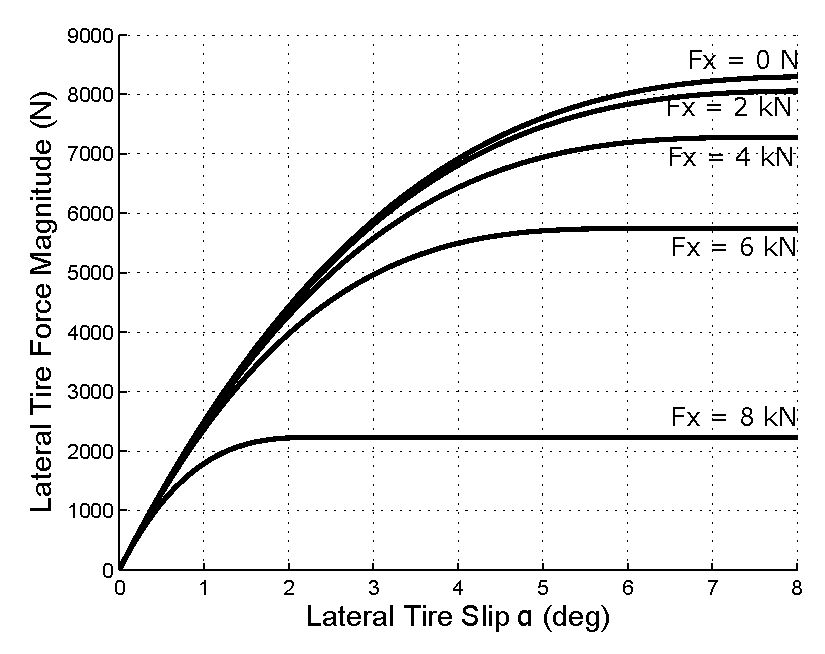
\includegraphics[width=.8\fullwidth]{tirecurves.eps}
\caption{Lateral tire force curve as a function of longitudinal force $F_x$ and lateral tire slip $\alpha$.}
\label{fig:coupledTires}
\end{figure} 

The next step is to break up the control inputs into the closed-loop feedback term and the \textit{learned} component that is
modified on every lap by the ILC algorithm:
\begin{align}
\label{eqn:splitTerms}
F_x &= F^{\mathrm{FB}}_x + F^L_x\\
    &= -K_xv + F^L_x\\
\delta &= \delta_{\mathrm{FB}} + \delta_L\\
\delta &= -k_p(e + x_\mathrm{LA}\Delta\Psi) + \delta_L
\end{align}
where $K_x$ is the proportional speed tracking gain and $k_p$ and $x_\mathrm{LA}$ are the lookahead gains discussed in Chapter 2. Note
that (\ref{eqn:splitTerms}) is similar to a feedback-feedforward control formulation. In fact, iterative learning control achieves
near-perfect reference tracking by refining the \textit{feedforward} control input to account for unmodeled dynamics and repeating disturbances that
affect the closed-loop controller performance. 

The closed loop system dynamics are now given by: 
\begin{align}
\label{eq:fullNLCL}	
	\frac{de}{dt} &= \left(v+U^\mathrm{des}_x(s)\right)(\beta + \Delta\Psi) \\
	\frac{dv}{dt} &= \left(v+U^\mathrm{des}_x(s)\right)\beta r + \frac{-K_xv + F^L_x}{m} - \frac{F_\mathrm{yf}(\alpha_F,F_x)-k_p(e + x_{LA}\Delta\Psi) + \delta_L}{m}\\
	\frac{d\beta}{dt} &= \frac{F_\mathrm{yf}(\alpha_\mathrm{f}, F_x) + F_\mathrm{yr}(\alpha_\mathrm{f},F_x)}{m\left(v + U^\mathrm{des}_x(s)\right) - r} \\
	\frac{dr}{dt}     &= \frac{aF_\mathrm{yf}(\alpha_\mathrm{f}, F_x) - bF_\mathrm{yr}(\alpha_\mathrm{r}, F_x)}{I_z} \\
	\frac{d\Delta\Psi}{dt} &= r
\end{align}
The nonlinear closed-loop dynamics must be converted into an affine, discrete-time dynamical system to apply conventional iterative learning
control algorithms. In our case, we have two system outputs ($y = [e \hspace{2mm} v]^T$) that are measured and two input signals to learn ($u = [\delta_L \hspace{2mm} F^L_x]^T$). 
Since we run the iterative learning control algorithm after seeing a trial of data, we can approximate
the dynamics in (\ref{eq:fullNLCL}) by linearizing about the observed states and inputs $x_o, u_o$ from the first lap. The affine model is therefore given by: 
 \begin{align}
 \label{eq:ssMAT}
 \begin{bmatrix} \dot{e} \\ \dot{\beta} \\ \dot{r} \\ \dot{\Delta\Psi} \\ \dot{v}\end{bmatrix} &= \begin{bmatrix} A(t) \end{bmatrix} \begin{bmatrix} e \\ \beta \\ r \\ \Delta\Psi \\ v \end{bmatrix} + \begin{bmatrix} B(t) \end{bmatrix} \begin{bmatrix} \delta_L \\ F^L_x \end{bmatrix} + d(t) \\
 \begin{bmatrix} \dot{e} \\ \dot{v} \end{bmatrix}  &= \begin{bmatrix} 1 & 0 & 0 & 0 & 0 \\ 0 & 0 & 0 & 0 & 1 \end{bmatrix} x
 \end{align}
 
 The time-varying state space matrices  where $A(t)$ and $B(t)$ are given by Jacobian linearizations of the closed loop nonlinear dynamics $f(x)$ (\ref{eq:fullNLCL}) about the observed states and inputs $x_o(t), u_o(t)$ from the last trial:
 \begin{align}
 \label{eq:C4nl}
 \begin{bmatrix} A(t) \end{bmatrix} &= \frac{\partial{f}}{\partial{x}}\Big|_{x_o(t)} \\
 \begin{bmatrix} B(t) \end{bmatrix} &= \frac{\partial{f}}{\partial{u}}\Big|_{u_o(t)}
 \end{align}
 While this multiple-input, multiple-output (MIMO) model captures the coupled behavior of the longitudinal and lateral inputs, it is tedious to compute,
 either numerically or analytically. For the case where the longitudinal and lateral inputs are decoupled, we obtain the same Chapter 2 linear state equations for the lateral
 dynamics: 
\begin{subequations}
\label{eq:bmC4}
\begin{align}
	\dot{\beta} &= \frac{F_\mathrm{yf}+F_\mathrm{yr}}{mU_x} - r \qquad \dot{r} = \frac{aF_\mathrm{yf} - bF_\mathrm{yr}}{I_z} \label{bm1} \\
	\dot{e} &= U_x (\beta + \Delta\Psi) \qquad \Delta\dot{\Psi} = r - U_x\kappa \label{eq:bm2} 
\end{align}
\end{subequations} 
and the following first order equation for the longitudinal dynamics, assuming a simple point mass model with proportional
speed tracking feedback:
\begin{equation}
\dot{v} = \frac{-K_xv + F^L_x}{m}
\end{equation}
The resulting state matrices $A(t)$ and $B(t)$ for (\ref{eq:ssMAT}) are then simply block diagonal matrices consisting of the
linearized lateral dynamics from Chapter 3 and the first order longitudinal dynamics:

\begin{align}
\label{eqn:C4dyn}
 A(t)  &= \begin{bmatrix}
  0 & U_x(t) & 0 & U_x(t) & 0\\ 
  0 & 0 & 1 & 0 & 0 \\ 
  \frac{-ak_\mathrm{p} \tilde{C}_\mathrm{f}(t)}{I_\mathrm{z}}  & \frac{-ak_\mathrm{p}x_\mathrm{LA}\tilde{C}_\mathrm{f}(t)}{I_\mathrm{z}}  & \frac{-a^2\tilde{C}_\mathrm{f}(t)-b^2\tilde{C}_\mathrm{r}(t)}{U_x(t)I_\mathrm{z}} & \frac{b\tilde{C}_\mathrm{r}(t) - a\tilde{C}_\mathrm{f}(t)}{I_\mathrm{z}} & 0 \\
  \frac{-k_\mathrm{p}\tilde{C}_\mathrm{f}(t)}{mU_x(t)}  & \frac{-k_\mathrm{p}x_\mathrm{LA}\tilde{C}_\mathrm{f}(t)}{mU_x(t)}  & \frac{b\tilde{C}_\mathrm{r}(t)-a\tilde{C}_\mathrm{f}(t)}{mU_x(t)^2}-1 & \frac{-\tilde{C}_\mathrm{f}(t) - \tilde{C}_\mathrm{r}(t)}{mU_x(t)} & 0 \\
  0 & 0 & 0 & 0 & -K_x 
  \end{bmatrix} \\
B(t) &=\begin{bmatrix} 0 & 0 \\	 	0 & 0 		\\ 		\frac{a \tilde{C}_\mathrm{f}(t)}{I_\mathrm{z}} & 0 		\\ 		\frac{\tilde{C}_\mathrm{f}(t)}{mU_x(t)} & 0 		\\ 0 & 1 \end{bmatrix} 
\end{align}
The affine term $d(t)$ is given by: 
\begin{align}
d(t) = \left[\begin{matrix} 0 \\
               -\kappa(t) U_x(t) \\ 
			    \frac{a\tilde{C}_\mathrm{f}(t)\tilde{\alpha}_\mathrm{f}(t) - b\tilde{C}_\mathrm{r}(t)\tilde{\alpha}_\mathrm{r}(t) + a\tilde{F}_\mathrm{yf}(t) - b\tilde{F}_\mathrm{yr}(t)}{I_z}\\
				\frac{\tilde{C}_\mathrm{f}(t)\tilde{\alpha}_\mathrm{f}(t) + \tilde{C}_\mathrm{r}(t)\tilde{\alpha}_\mathrm{r}(t) + \tilde{F}_\mathrm{yf}(t) + \tilde{F}_\mathrm{yr}(t)}{mU_x(t)}\\
				0 \\
				0
				\end{matrix}\right]
\end{align}
While (\ref{eqn:C4dyn}) is written as a MIMO system for compactness, assuming decoupled lateral and longitudinal 
dynamics provides two single-input, single-output (SISO) systems. 

\newpage
\section{Lifted Domain Representation and ILC \newline Problem Statement}
\label{sec:liftedD}
Whether the coupled (\ref{eq:C4nl}) or decoupled (\ref{eqn:C4dyn}) dynamics are assumed, the
final modeling step is to apply standard discretization techniques to obtain dynamics in the following form:
\begin{align}
\label{C4ad}
x_{k+1} &= A_kx_k + B_ku_k + d_k \\
y_{k}   &= Cx_k
\end{align}
For a given lap of racing $j$, sensor measurements provide $N$ observations of both the lateral path deviation $e$ and longitudinal
speed tracking error $v$. These measurements can be stacked into a 2$N \times 1$ array: 
\begin{equation}
\mathbf{e}_j = \begin{bmatrix} e_1 & \hdots & e_N & v_1 & \hdots & v_N \end{bmatrix}^T
\end{equation} 
These measurement errors are related to the learned control inputs $\delta^L$ and $F^L_x$ as follows: 
\begin{align}
\label{eq:liftedDomain}
\mathbf{e}_j &= P\mathbf{u}^L_j + \mathbf{w} \\
\mathbf{u}^L_j &= \begin{bmatrix} \delta^L_1 & \hdots & \delta^L_N & F^L_{x1} & \hdots & F^L_{xN} \end{bmatrix}^T
\end{align}
The system dynamics modeled in the previous section are represented by the \textit{lifted-domain} dynamics matrix $P$,
which is $\mathrm{2}N \times \mathrm{2}N$ and given by:
\begin{equation}
\label{eq:C4bm}
P=\left[
\begin{array}{c|c}
P_{e\delta} & P_{eF} \\ \hline
P_{v\delta} & P_{vF} 
\end{array}\right]
\end{equation}
Where each submatrix in (\ref{eq:C4bm}) is $N \times N$ and represents the lifted-domain dynamics from a given input to a given output. 
Individual terms of the sub-matrices are given by:

\begin{equation}
\label{eq:how2Lift}
p_{lk} = \begin{cases} 0 &\mbox{if } l < k \\ 
C_yB_u(k) & \mbox{if } l = k \\
C_yA(l)A(l-1)\cdots A(k)B_u(k) &\mbox{if } l > k \end{cases}
\end{equation} 
Where $C_y$ is the row of $C$ in (\ref{C4ad}) corresponding to the desired output and $B_u$ the column of $B$ in (\ref{C4ad})
corresponding to the desired input. Note that
for the case of uncoupled lateral and longitudinal dynamics, the off-diagonal sub-matrices of $P$ are $[0]$ since we have
two SISO systems. The term $\mathbf{w}$ in (\ref{eq:liftedDomain}) is the unknown disturbance. Iterative
learning control relies on the assumption that this disturbance is the underlying cause of the observed errors $\mathbf{e}_j$, and that 
the disturbance, while unknown, is constant from lap to lap.

Given the error signal $\mathbf{e}_j$ for a given lap $j$, the iterative learning problem is to find the inputs $\mathbf{u}_{j+1}$ that
will cancel out the tracking error on the next lap. The learned inputs are then applied, the observed error $\mathbf{e}_{j+1}$ is recorded,
and the process is repeated until the tracking error falls to a desired level. There is a wide body of literature on methods to determine $\mathbf{u}_{j+1}$ given $P$ and $\mathbf{e}_j$, but this dissertation will
investigate the most common approach. We compute the ILC input for the next lap with the following formulation:

\begin{align}
 \label{eqn:ctrlLaw}
 \mathbf{u}^L_{j\!+\!1} = Q(\mathbf{u}^L_j - L\mathbf{e}_j)
\end{align}
where $Q$ is the $2N \times 2N$ \textit{filter} matrix, and $L$ is the $2N \times 2N$ \textit{learning} matrix. 
In the following two sections, the
matrices $Q$ and $L$ will be obtained by designing a proportional-derivative (PD) iterative learning controller as well as a quadratically
optimal (Q-ILC) learning controller.

\newpage
\section{Proportional-Derivative Controller}
\label{sec:pdcontroller}

The proportional-derivative ILC computes the steering $\delta^L$ and force $F^L$ correction for the current lap $j$ based on the error and 
error derivative at the same time index $k$ from the previous lap:
\begin{align}
	\label{eq:PDlaw}
	\delta^L_{j}(k) &= \delta^L_{j\!-\!1}(k) - k_{p\delta}e_{j\!-\!1}(k) - k_{d\delta}(e_{j\!-\!1}(k) - e_{j\!-\!1}(k-1))\\
	    F^L_{j}(k) &=  F^L_{j-1}(k) - k_{pF}v_{j\!-\!1}(k) - k_{dF}(v_{j\!-\!1}(k) - v_{j\!-\!1}(k-1))
\end{align}
where $k_{p\delta}$ and $k_{pF}$ are proportional gains and $k_{d\delta}$ and $k_{dF}$ are derivative gains. In the lifted domain representation from (\ref{eqn:ctrlLaw}), the resulting learning matrix $L$ is given by
\begin{equation}
	L = \begin{bmatrix} 		-(k_{p\delta}+k_{d\delta}) &          &  0                            & 0 & \hdots & 0 \\ 
									   k_{d\delta}                     &  \ddots  &                               & \vdots & \ddots & \vdots\\ 
									   0                       &   k_{d\delta}    &    -(k_{p\delta}+k_{d\delta}) & 0 & \hdots & 0 \\
						               0 & \hdots & 0 & -(k_{pF}+k_{dF}) &          &  0\\
									   \vdots & \ddots & \vdots & k_{dF} &  \ddots  &                               &\\
									   0 & \hdots & 0  & 0 & k_{dF} & -(k_{pF} + k_{dF}) \\			
			\end{bmatrix}
\end{equation}
 
 The PD equation (\ref{eq:PDlaw}) determines $\delta^L$ only using lateral path deviation $e$ and $F^L_x$ using only the speed tracking error $v$. Since
 we have formulated the problem as a MIMO system, it is possible to generalize and have both inputs depend on both outputs, but this is not considered for 
 simplicity of gain selection. The filter matrix $Q$ is obtained by taking any filter transfer function and converting into the lifted domain via (\ref{eq:how2Lift}).
 An important design consideration in choosing the two $k_p$ and $k_d$ gains is avoiding a poor lap-to-lap
``transient" response, where the path tracking error increases rapidly over the first several laps before
eventually decreasing to a converged error response $e_\infty$. This is a commonly encountered design requirement
for ILC systems, and can be solved by ensuring the following \textit{monotonic convergence} condition is met \cite{bristow}:

\begin{equation}
	\gamma \triangleq \bar{\sigma}(PQ(I-LP)P^{-1}) < 1
	\label{eq:MS}
\end{equation}
where $\bar{\sigma}$ is the maximum singular value. In this case, the value of $\gamma$ provides an upper bound on the change
 in the tracking error norm from lap to lap, i.e. 
 
\begin{equation}
	||\mathbf{e}_\infty - \mathbf{e}_{j+1}||_2 \leq \gamma ||\mathbf{e}_\infty-\mathbf{e}_j||_2
\end{equation}

Fig.~\ref{fig:stabPlot} shows values of $\gamma$ for both an unfiltered PD controller ($Q = I$), and for a PD controller with a 2 Hz, first order low pass filter. The $\gamma$ values are plotted as a
contour map against the controller gains $k_{p\delta}$ and $k_{d\delta}$. Addition of the low-pass filter
assists with monotonic stability by removing oscillations in the control input generated when trying to remove small reference tracking
errors after several iterations. Since the filtering occurs when generating a control signal for the next lap, the filter $Q$ can be zero-phase. 
The plot shown in Fig.~\ref{fig:stabPlot} is for the steering ILC design only, but the same analysis is possible for the longitudinal
ILC design as well. The stability analysis in Fig.~\ref{fig:stabPlot} assumes the $P$ 
matrix is constant for all iterations and is generated assuming decoupled vehicle dynamics
 for a straight-line trajectory at a constant speed of 20 m/s. Because the $P$ matrix in general can change from iteration to iteration and will also
 change depending on the trajectory, making a general assertion or proof about stability of the iterative learning controller is difficult. 

\begin{figure}[tb]
\centering
\includegraphics[width=.7\fullwidth]{MonotonicStability.png}
\caption[Values of convergence bound $\gamma$ vs. $k_{p\delta}$ and $k_{d\delta}$ for PD iterative learning controller]{Values of convergence bound $\gamma$ vs. $k_{p\delta}$ and $k_{d\delta}$ for PD iterative learning controller with (top) no filtering and (bottom) with a 2 Hz low-pass filter. Lower values of $\gamma$ correspond to faster convergence.
Shaded regions correspond to gains that result in system monotonic stability. }
\label{fig:stabPlot}
\end{figure}


\section{Quadratically Optimal Controller}\label{sec:controller}
\label{sec:qopt}
An alternate approach to determining the learned steering and longitudinal force input is to minimize a quadratic cost function for the next lap:

\begin{align}
J_{j\!+\!1} = \textbf{e}_{j\!+\!1}^TT\textbf{e}_{j\!+\!1} + \textbf{u}^T_{j\!+\!1} R \textbf{u}^T_{j\!+\!1}+\Delta_{j\!+\!1}^TS\Delta_{j\!+\!1}
\label{eq:QILC}
\end{align}
where $\Delta_{j\!+\!1} = \mathbf{u}^L_{j\!+\!1} - \mathbf{u}^L_j$ and the $2N \times 2N$ matrices $T$, $R$, and $S$ are weighting matrices, each given
by a scalar multiplied by the identity matrix for simplicity.
This formulation allows the control designer to weight the competing objectives of minimizing the tracking errors $e$ and $v$, control effort $|\delta^L|$ and $|F^L_x|$, and change in the control signal from lap to lap.
While constraints can be added to the optimization problem, the unconstrained problem in (\ref{eq:QILC}) can be solved analytically \cite{bristow2008} to obtain desired controller and filter matrices:

\begin{subequations}
\label{eq:analSol}
\begin{align}
	Q &= (P^TTP + R + S)^{-1}(P^TTP + S)\\
	L &= (P^TTP + S)^{-1}P^TTP(T^{1/2}P)^{-1}T^{1/2}
\end{align}
\end{subequations}

An advantage of the quadratically optimal control design over the simple PD controller is that the controller matrices $Q$ and $L$ take the linearized, time-varying dynamics $P$ into account. 
This allows the iterative learning algorithm
to take into account changes in the steering dynamics due to changes in vehicle velocity.
Furthermore, if the fully coupled dynamics (\ref{eq:C4nl}) are used, the iterative learning algorithm also accounts for the
second-order effect of steering on the longitudinal dynamics and longitudinal force application on the lateral dynamics. 
 However, a disadvantage is that computing $\mathbf{\delta}^L$ in (\ref{eqn:ctrlLaw}) requires matrix multiplications with
the typically dense matrices $Q$ and $L$ for every lap, which can be computationally expensive for fast sampling rates. 

\section{Simulated Results}
\label{sec:simres}

To test the feasibility of the PD and Q-ILC learning algorithms, the vehicle tracking performance over multiple laps is
simulated using the path curvature and speed profiles shown in Fig.~\ref{fig:simSetup}. To test the performance
of the controller at varying accelerations, four speed profiles are tested. Each profile is
generated with a different level of peak combined longitudinal/lateral acceleration, ranging from 5 $\mathrm{m/s^2}$ (below the limits)
up to 9.5 $\mathrm{m/s^2}$ (close to exceeding the limits). For accurate results, simulations were conducted using numerical integration with
 fully nonlinear equations of motion (\ref{eq:fullNL})-(\ref{eq:fullNL2}) and coupled lateral/longitudinal dynamics \cite{rami}.

\begin{figure}[bh]
\centering
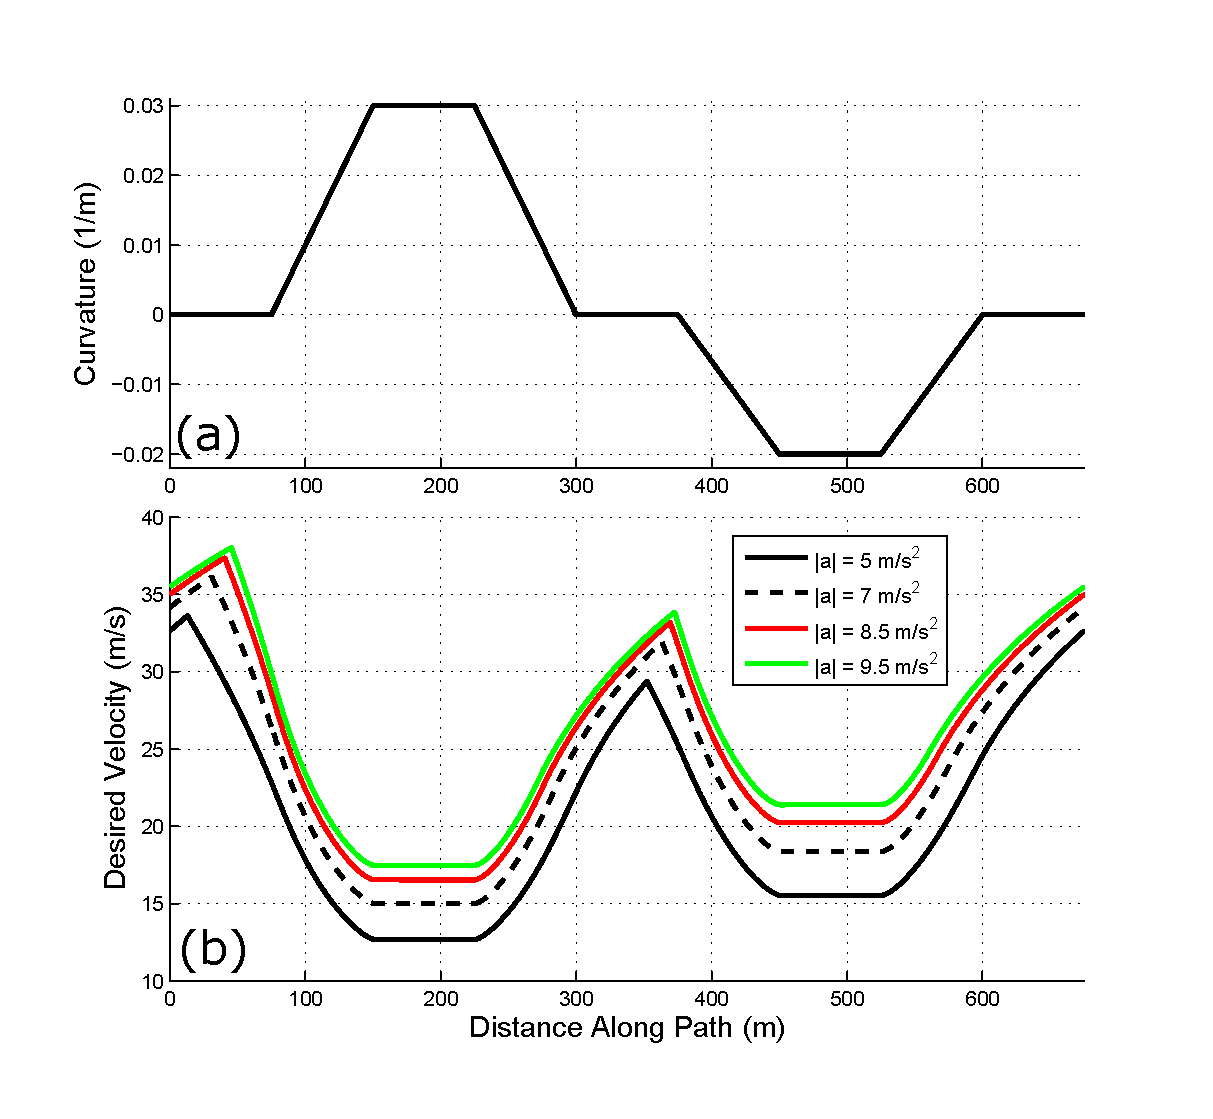
\includegraphics[width= .88\fullwidth]{simSetup.eps}
\caption[Curvature profile used for ILC simulation.]{ (a) Curvature profile used for ILC simulation. (b) Velocity profiles generated for four different levels of longitudinal/lateral acceleration. }
\label{fig:simSetup}
\end{figure}

Simulated results for the root-mean-square (RMS) lateral path deviation is shown in Fig.~\ref{fig:simRes1}. The results
show the change in RMS error as the number of ILC iterations increase. Three different ILC controllers are tested. 
The first controller is the simple PD controller
with low-pass filter (\ref{eq:PDlaw}), and the second controller is the quadratically optimal ILC algorithm (\ref{eq:analSol}) assuming fully coupled dynamics (\ref{eq:C4nl}) in the plant
matrix $P$ (i.e. the full MIMO system).
The third controller is also the quadratically optimal ILC algorithm, but the $P$ matrix used in the optimization
assumes decoupled dynamics (\ref{eqn:C4dyn}) and therefore solves the lateral and longitudinal SISO problems separately. 

\begin{figure}[h!]
\centering
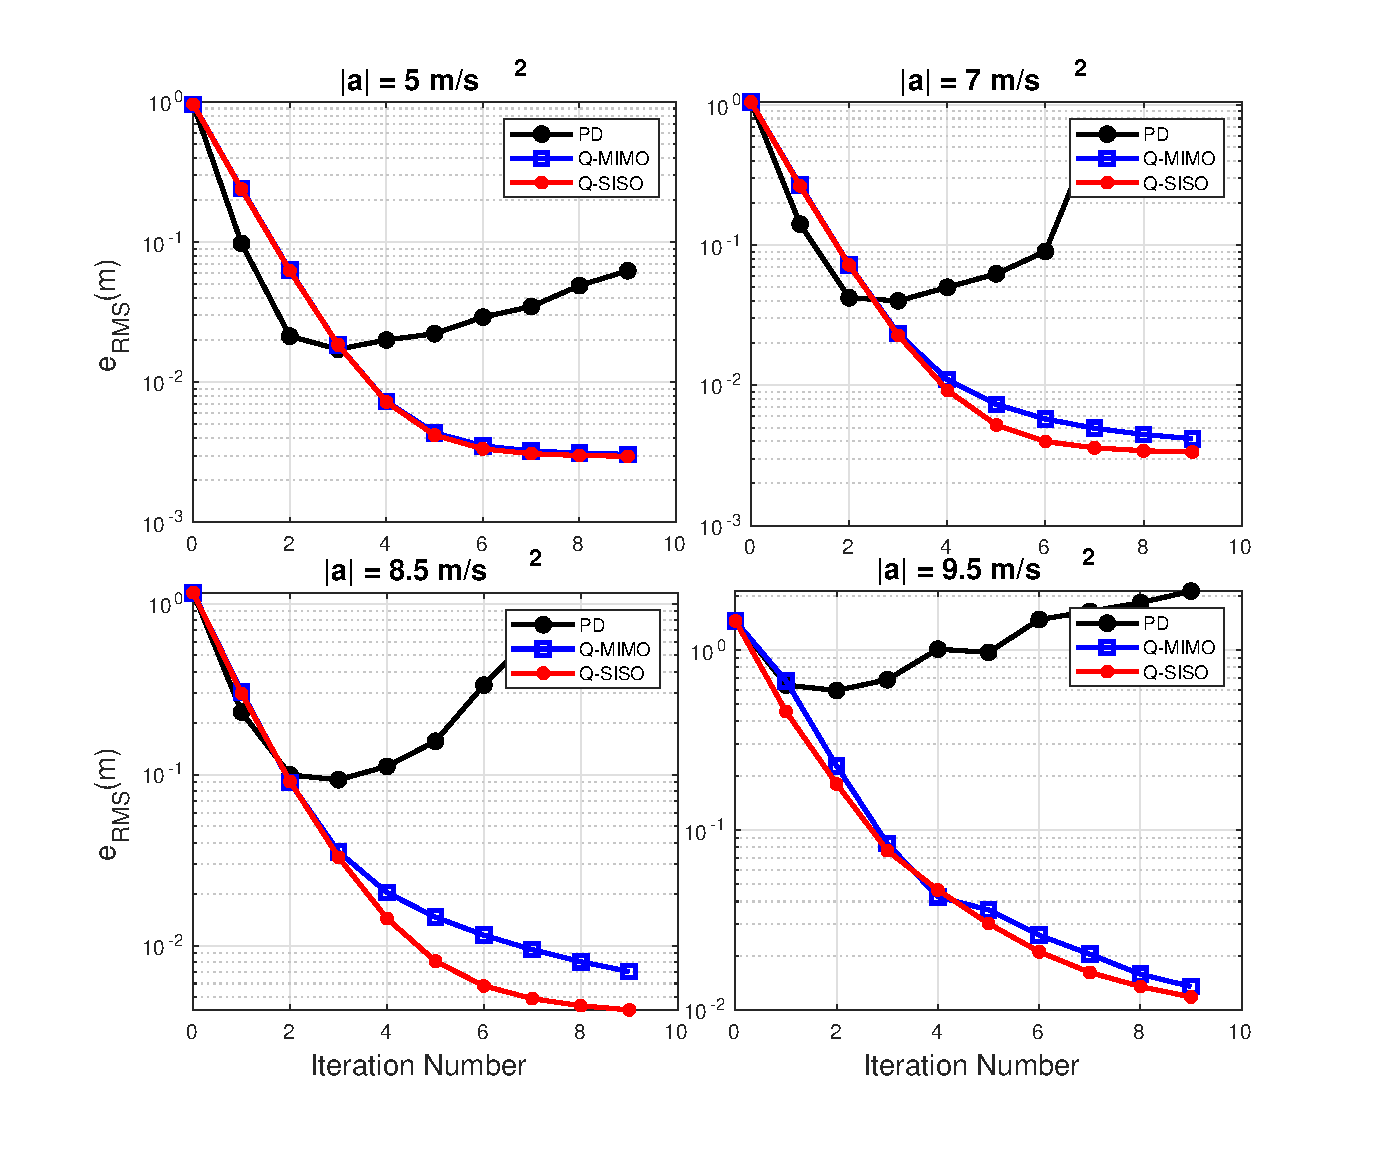
\includegraphics[width=.92\fullwidth]{simRes1.eps}
\caption[Simulated results for root-mean-square path tracking error at several values of vehicle acceleration]{Simulated results for root-mean-square path tracking error at several values of vehicle acceleration, with $T = R = I$ and $S = \mathrm{100} I$.
Results are plotted on a log scale.}
\label{fig:simRes1}
\end{figure}

Fig.~\ref{fig:simRes1} shows that both quadratically optimal ILC algorithms exponentially reduce the lateral
path tracking error as the number of learning iterations is increased. Overall, the RMS lateral tracking performance is
better at lower vehicle accelerations. This is unsurprising for two reasons. In Chapter 2, we discovered that lateral path deviation in 
general increases for the lookahead steering feedback at higher accelerations. Second, our estimate of the vehicle dynamics contained in $P$
is based on linearization, and the vehicle dynamics at lower accelerations are mostly linear.

Fig.~\ref{fig:simRes2} shows the same results as Fig.~\ref{fig:simRes1}, but for the speed tracking performance. 
The overall trends are very similar. In both plots, there is very little difference between the coupled MIMO formulation and decoupled SISO 
formulation at low accelerations. This is expected, as the longitudinal and lateral dynamics are independent when the vehicle tires are not saturated.
At higher accelerations, there are small differences, but the overall RMS errors are still quite similar. A reason for this is the
nature of the speed profiles in Fig.~\ref{fig:simSetup}. The vehicle spends the majority of time either fully braking/accelerating or
turning at a constant velocity. There are only a few small transient regions where the vehicle needs significant amounts of both 
lateral and longitudinal acceleration. As a result, the need to account for the coupled dynamics may not be important in practice, especially
given the larger computation time needed when $P$ is dense and not block-diagonal.     

\begin{figure}[tb]
\centering
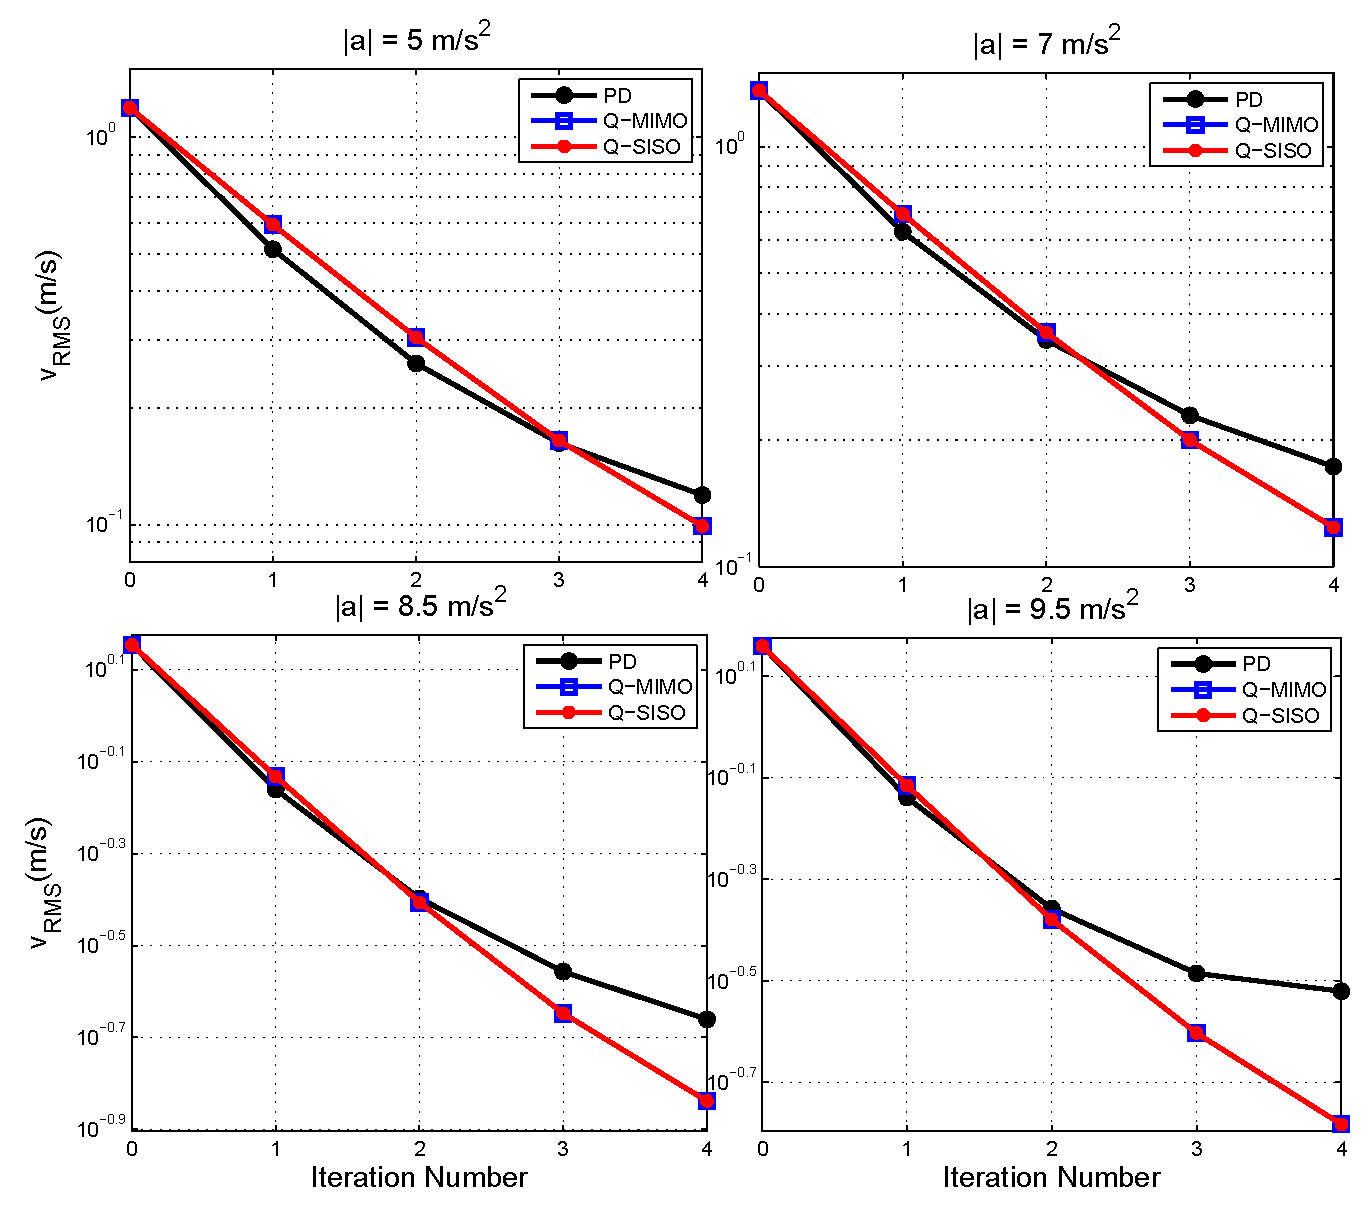
\includegraphics[width=\fullwidth]{simRes2.eps}
\caption[Simulated results for root-mean-square speed tracking error $v$ at several values of vehicle acceleration.]{Simulated results for root-mean-square speed tracking error $v$ at several values of vehicle acceleration, with $T = I$, $R = 0$, and $S = \mathrm{1e-7} I$.
Results are plotted on a log scale.}
\label{fig:simRes2}
\end{figure}

A final comment is that the proportional-derivative ILC algorithm performs relatively poorly. At low accelerations, the
speed and path tracking performance both improve initially, but fail to improve after the second learning iteration. At high
lateral and longitudinal accelerations, the tracking performance becomes even worse for the steering ILC in Fig.~\ref{fig:simRes1}.  
This is unsurprising given that the linearized plant dynamics $P$ are not explicitly accounted for in the selection of the PD gains. 
While the point mass model for the longitudinal dynamics is a relatively simple first order model, the lateral dynamics 
are fourth order and highly speed dependent. A simple PD approach for learning control is likely insufficient at the limits of handling
without a more sophisticated set of PD gains for different vehicle speeds.

\section{Experimental Results}
\label{sec:ch4ExpRes}

Experimental data for iterative learning control was collected over four laps at Thunderhill Raceway with the autonomous Audi TTS
setup described in Chapters 2 and 3. The experimental controller setup is shown in Fig.~\ref{fig:C4setup}, and controller parameters are shown in Table \ref{tb:ilcprm}. 

\begin{figure}[h]
\centering
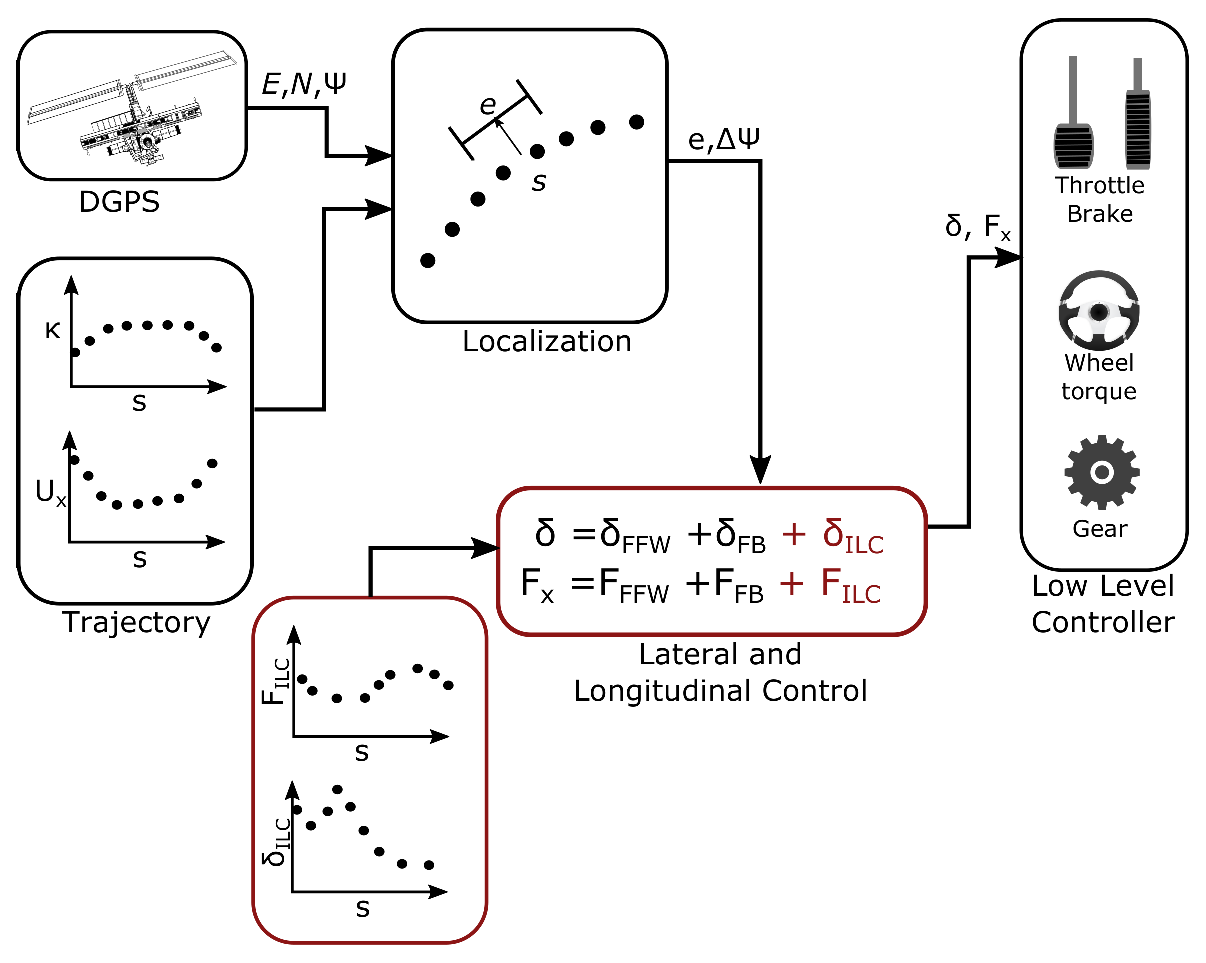
\includegraphics[width=\fullwidth]{expSetupC4.eps}
\caption{Controller setup for experimental testing of iterative learning control.}
\label{fig:C4setup}
\end{figure}

\newpage
The key difference between the controller setup from Chapter 3 is the inclusion of the learning inputs $\delta^L$ and $F^L_x$. To save
computation time, these are calculated at a 10 Hz update rate at the end of every race lap and stored as lookup tables in the controller. 
Since the the real-time control occurs at 200 Hz, at every time step the controller interpolates
the lookup table and applies the correct force and steer angle correction. One key difference between the simulation and
the experiment is that the simulation only applied the learning correction to the closed-loop path tracking controller. 
In the experiment, the steady-state feedforward
 control laws from Chapter 2 are also applied to keep the tracking error on the first lap below 1 m for safety. 
 
\begin{table}[tb]
\begin{center}
\caption{Vehicle Parameters}\label{tb:ilcprm}
\begin{tabular}{lccc}
Parameter & Symbol & Value & Units \\\hline
Lookahead Distance       & $x_\mathrm{LA}$          &  15.2 & $\mathrm{m} $ \\
Lanekeeping Gain         & $k_{\mathrm{LK}}$         & 0.053 & $\mathrm{rad\,m^{-1}}$\\
Lanekeeping Sample Time  & $t_s$                        & 0.005 & s\\
ILC Sample Time          & $T_s$                        & 0.1   & s\\
Speed Tracking Gain                & $K_x$           & 2500 & $\mathrm{Nsm^{-1}}$\\
Q-ILC Matrix (Path)            & $T$ and $R$              &  $I$      & - \\
Q-ILC Matrix  (Path)           & $S$                       & 100\,$I$  & - \\
Q-ILC Matrix (Speed)            & $T$              &  $I$      & - \\
Q-ILC Matrix (Speed)            & $R$              &  $0$      & - \\
Q-ILC Matrix  (Speed)           & $S$                       & 1e-7\,$I$  & - \\\hline
\end{tabular}
\end{center}
\end{table}


Fig.~\ref{fig:expRes1} shows the applied iterative learning signals and resulting path tracking error over four laps using the SISO
quadratically optimal learning algorithm. The car is driven
aggressively at peak lateral/longitudinal accelerations of 8 $\mathrm{m/s^2}$. On the first lap, despite the 
incorporation of a feedforward-feedback controller operating at a high sampling rate, several spikes in tracking error are visible due to transient
vehicle dynamics neglected by the feedforward controller design from Chapter 2.

However, the iterative learning algorithm is able to significantly attenuate these transient spikes after just two or three laps. 
One of the most important features of the time series plot is that the learned steering corrections are applied slightly before a lateral
path deviation was observed the prior lap (i.e. the steering corrections \textit{lead} the observed error). This is because the learning
algorithm has knowledge of the system model and knows that a steering correction must be applied a few meters early to cancel a path deviation
further down the road.

\begin{figure}[h!]
\centering
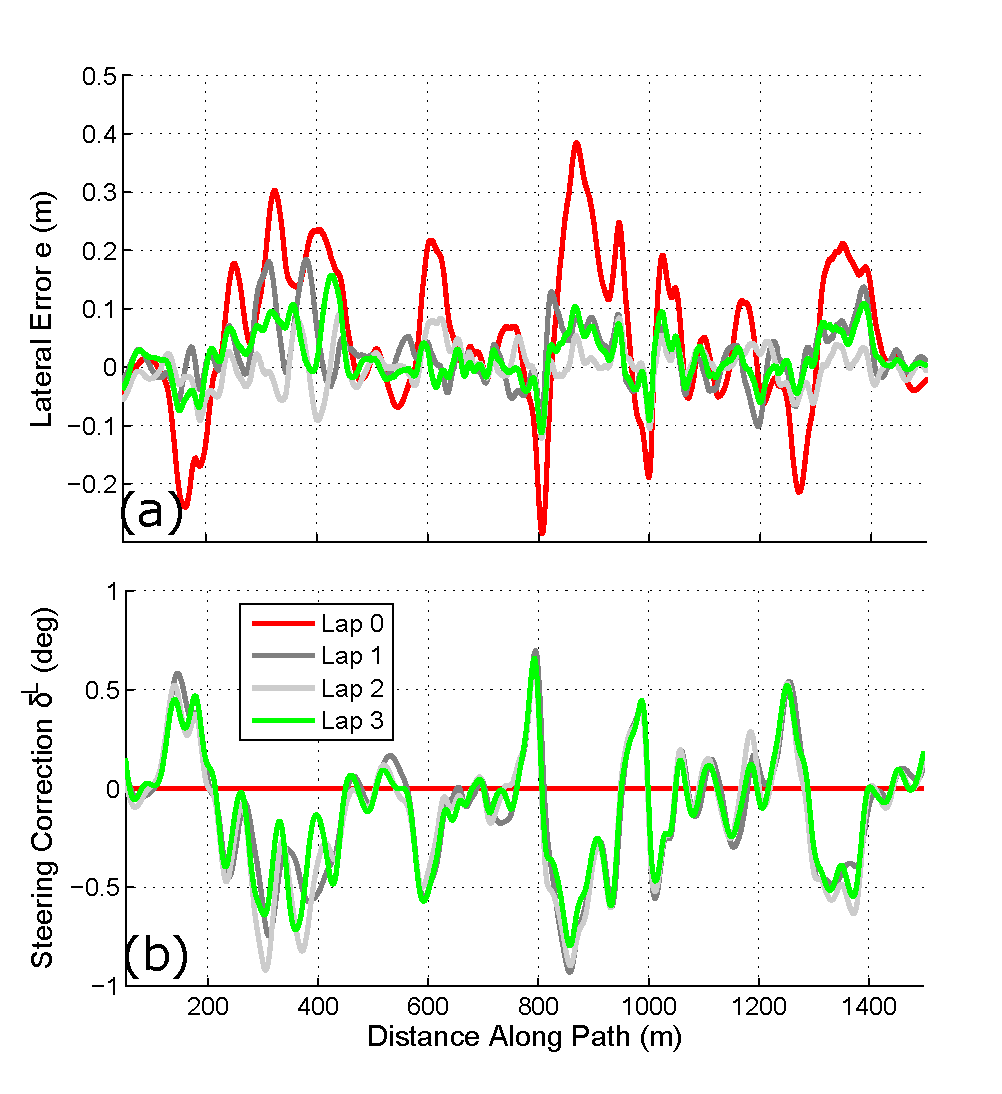
\includegraphics[width=\fullwidth]{expRes1.eps}
\caption{Experimental results for path tracking error with Q-SISO learning controller, at peak lateral accelerations of 8 $\mathrm{m/s^2}$.}
\label{fig:expRes1}
\end{figure}

\begin{figure}
\centering
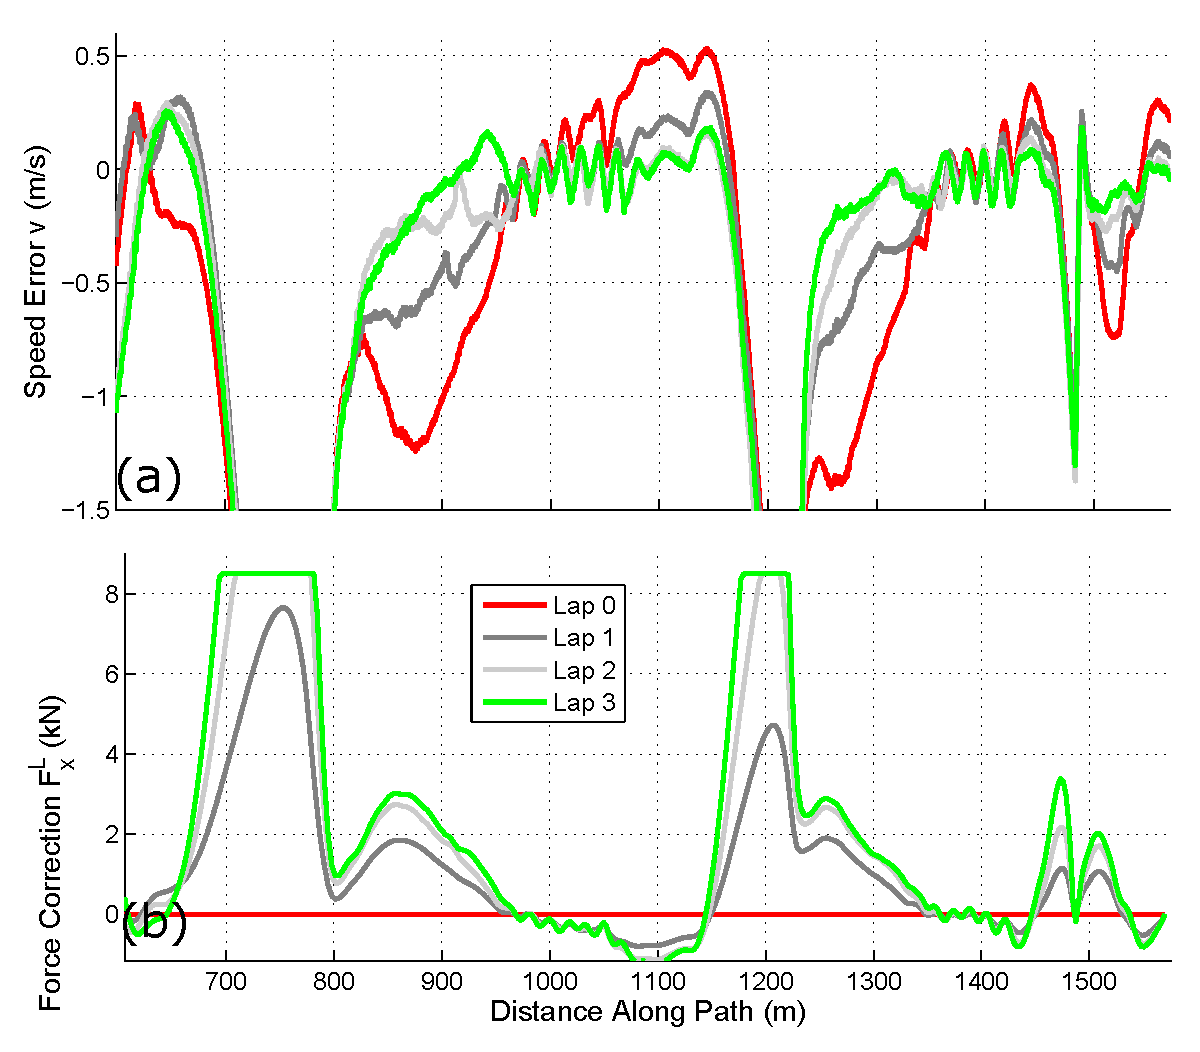
\includegraphics[width=.95\fullwidth]{expRes2.eps}
\caption{Experimental results for speed tracking error with Q-SISO learning controller, at peak lateral accelerations of 8.5 $\mathrm{m/s^2}$.}
\label{fig:expRes2}
\end{figure}
Fig.~\ref{fig:expRes2} shows the iterative learning signals for the longitudinal speed control at a slightly
higher acceleration of 8.5 $\mathrm{m/s^2}$. Again, in just
two to three iterations, significant lags in the speed tracking are attenuated from $s = 800-900$ meters and $s = 1200-1300$ meters. Additionally, the controller also acts to slow the car down when $v > 0$ and the vehicle exceeds the speed profile. This is also desirable
from a racing perspective as it it prevents the vehicle from exceeding the friction limit. Oscillations in speed tracking
performance are visible in Fig.~\ref{fig:expRes1}(a) from 900 - 1100 meters and 1300 - 1400 meters. These are generally undesirable, and further tuning of the filter matrix $Q$ is possible
to remove rapid changes in the learned force input. 
 
 Notice that Fig.~\ref{fig:expRes2} has
several regions where the speed error $v << 0$. These are straight regions of the track where is no true planned speed
because the desired longitudinal action is to fully apply the throttle and go as fast as physically possible. For convenience, the ILC is programmed to saturate the longitudinal
learning signal to 8000 Newtons, although a more elegant solution is to switch the ILC controller off on straight portions of the track. 

In Fig.~\ref{fig:expRes3}, root-mean-square tracking results are shown for a range of peak vehicle accelerations. 
The results show that at lower vehicle accelerations,
the initial speed and lateral tracking errors (Iteration 0) are smaller, as the built-in feedback-feedforward controller 
performs better. However, as the speed profile becomes more aggressive, the path and speed tracking degrades in the presence
of highly transient tire dynamics. Regardless of the initial error, application of iterative learning control 
reduces the trajectory tracking errors significantly over just 2 or 3 laps. At an acceleration of 8.5 $\mathrm{m/s^2}$, for example, the RMS
lateral tracking error is around 3 cm, on the order of the expected RMS error from the GPS position sensor! 
On some tests, the RMS tracking error 
occasionally increases slightly from
Lap 2 to Lap 3, and for the case where vehicle acceleration is 9 $\mathrm{m/s^2}$, the lateral tracking error is constant from Lap 1 to Lap 2
before decreasing further in Lap 3. While not predicted in simulation, this behavior likely occurs because the repeating disturbance
from lap-to-lap is not exactly constant, especially as the vehicle approaches the handling limits. More refined tuning of the gain matrices may be able to prevent 
this RMS error increase, or the ILC algorithm can be stopped after several iterations once the tracking performance is acceptable.

Experimental results in this section were only given for the quadratically optimal controller with decoupled (SISO) dynamics. 
The PD iterative learning controller was not tested due to the relatively worse simulation performance, and the quadratically optimal 
controller with coupled dynamics provided no clear benefit in simulation but a much longer computation time. 



\begin{figure}
\centering
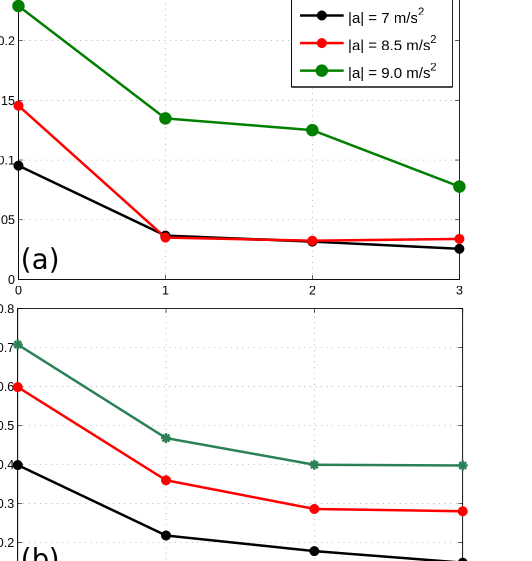
\includegraphics[width=.8\fullwidth]{expRes3.eps}
\caption[Experimental RMS tracking error for the Q-SISO learning controller at several levels of lateral acceleration. ]{Experimental RMS tracking error for the Q-SISO learning controller at several levels of lateral acceleration. (a) RMS lateral tracking
error as a function of lap number/iteration number. (b) RMS speed tracking error as a function of lap/iteration number. Note that lap 0 corresponds
to the baseline case where iterative learning control is not applied.}
\label{fig:expRes3}
\end{figure}

\section{Conclusion}

This chapter demonstrated the application of iterative learning control (ILC) methods to achieve accurate trajectory
following for an autonomous race car over multiple laps. Two different algorithms, proportional-derivative (PD) and 
quadratically optimal (Q-ILC) learning control are tested in simulation and then used to experimentally 
eliminate path tracking errors caused by the transient nature of the vehicle dynamics near the limits of friction. 

The primary significance of this work is improved racing performance of the autonomous vehicle over time. Because the vehicle lateral
and longitudinal dynamics become difficult to accurately model at the limits of handling, following a minimum-time speed and curvature
profile is difficult to achieve over one lap with a standard feedback control system. However, because the desired trajectory and vehicle
conditions are relatively unchanged on each subsequent lap, the presented ILC algorithms ensure accurate tracking of the minimum-time trajectory 
after just two or three laps of learning. 

One drawback with  iterative learning control is that applying a steering wheel input to eliminate
lateral errors will work only if the vehicle is near the limits of handling, but has not fully saturated the available tire forces on the front axle and entered a limit understeer condition.
Recall from \S \ref{sec:osteerusteer} that since the steering actuator of a vehicle only has direct control of the front tire forces, 
 additional turning of the steering wheel cannot reduce the vehicle's turning radius when the front axle is saturated.
In the next chapter, a separate learning algorithm is developed to learn the best velocity profile that minimizes lap time by
maximizing the available tire friction on all turns of the track.

\textit{Note: This chapter reuses material previously published by the author in \cite{kapaniaacc}.}



%\addtolength{\textheight}{-2cm}   % This command serves to balance the column lengths
                                  % on the last page of the document manually. It shortens
                                  % the textheight of the last page by a suitable amount.
                                  % This command does not take effect until the next page
                                  % so it should come on the page before the last. Make
                                  % sure that you do not shorten the textheight too much.


                                  


 